\documentclass[sigconf,nonacm]{acmart}
\usepackage[frozencache=true]{minted}
\usepackage{tikz} % for figures
\usetikzlibrary{arrows.meta,shapes.geometric}

\hyphenation{time-stamp time-stamps re-con-cilia-tion data-center}

\begin{document}
\title{Thinking in Events: From Databases to Distributed Collaboration Software}
\subtitle{Keynote at the 15th ACM International Conference on Distributed and Event-Based Systems (DEBS)}

\author{Martin Kleppmann}
\orcid{0000-0001-7252-6958}
\affiliation{%
  \institution{University of Cambridge}
  \city{Cambridge}
  \country{UK}
}
\email{mk428@cst.cam.ac.uk}

\begin{abstract}
TODO: Abstract
\end{abstract}

\begin{CCSXML}
<ccs2012>
  <concept>
    <concept_id>10002951.10002952.10002953.10010820.10003208</concept_id>
    <concept_desc>Information systems~Data streams</concept_desc>
    <concept_significance>500</concept_significance>
  </concept>
  <concept>
    <concept_id>10011007.10010940.10010971.10010972.10010975</concept_id>
    <concept_desc>Software and its engineering~Publish-subscribe / event-based architectures</concept_desc>
    <concept_significance>500</concept_significance>
  </concept>
  <concept>
    <concept_id>10010405.10010406.10010422</concept_id>
    <concept_desc>Applied computing~Event-driven architectures</concept_desc>
    <concept_significance>300</concept_significance>
  </concept>
  <concept>
    <concept_id>10003752.10003753.10003761.10003763</concept_id>
    <concept_desc>Theory of computation~Distributed computing models</concept_desc>
    <concept_significance>300</concept_significance>
  </concept>
</ccs2012>
\end{CCSXML}

\ccsdesc[500]{Information systems~Data streams}
\ccsdesc[500]{Software and its engineering~Publish-subscribe / event-based architectures}
\ccsdesc[300]{Applied computing~Event-driven architectures}
\ccsdesc[300]{Theory of computation~Distributed computing models}

\keywords{stream processing, event sourcing, CRDTs, state machine replication}
\maketitle

\def\figureautorefname{Figure}
\def\sectionautorefname{Section}
\def\subsectionautorefname{Section}
\def\subsubsectionautorefname{Section}

% Title: Event-based thinking in collaboration software

% What do Google Docs and stream processing have in common? Both are centered around the idea of streams of events. In the case of Google Docs and other collaboration software, each event describes a change that a user has made to a document. Each user's local device has a copy of the shared document, and processing the stream of changes means updating this local copy so that it is consistent with all of the other users' copies of the document.

% This talk will explore collaboration software through the lens of event-based thinking, explaining some of the algorithms that are used to implement this kind of software, such as Conflict-free Replicated Data Types (CRDTs). We will highlight new developments in this area, such as local-first software, and identify some open challenges in the area.

\section{Introduction}

TODO: Introduction

\section{A Taxonomy of Event-based Systems}\label{sec:taxonomy}

The term \emph{event} is used in many different ways in different branches of computing.
Many authors talk about events without always being explicit about the exact context they are referring to.
In order to facilitate a precise discussion of the trade-offs, I present a taxonomy that categorises the different uses of events, based on the flowchart in \autoref{fig:flowchart}.
Such a broad-brush taxonomy cannot necessarily capture all of the nuance of the field, and sometimes the boundaries between categories can be blurry.
Nevertheless, I hope that it will be a useful tool for structuring discussions.

\begin{figure*}
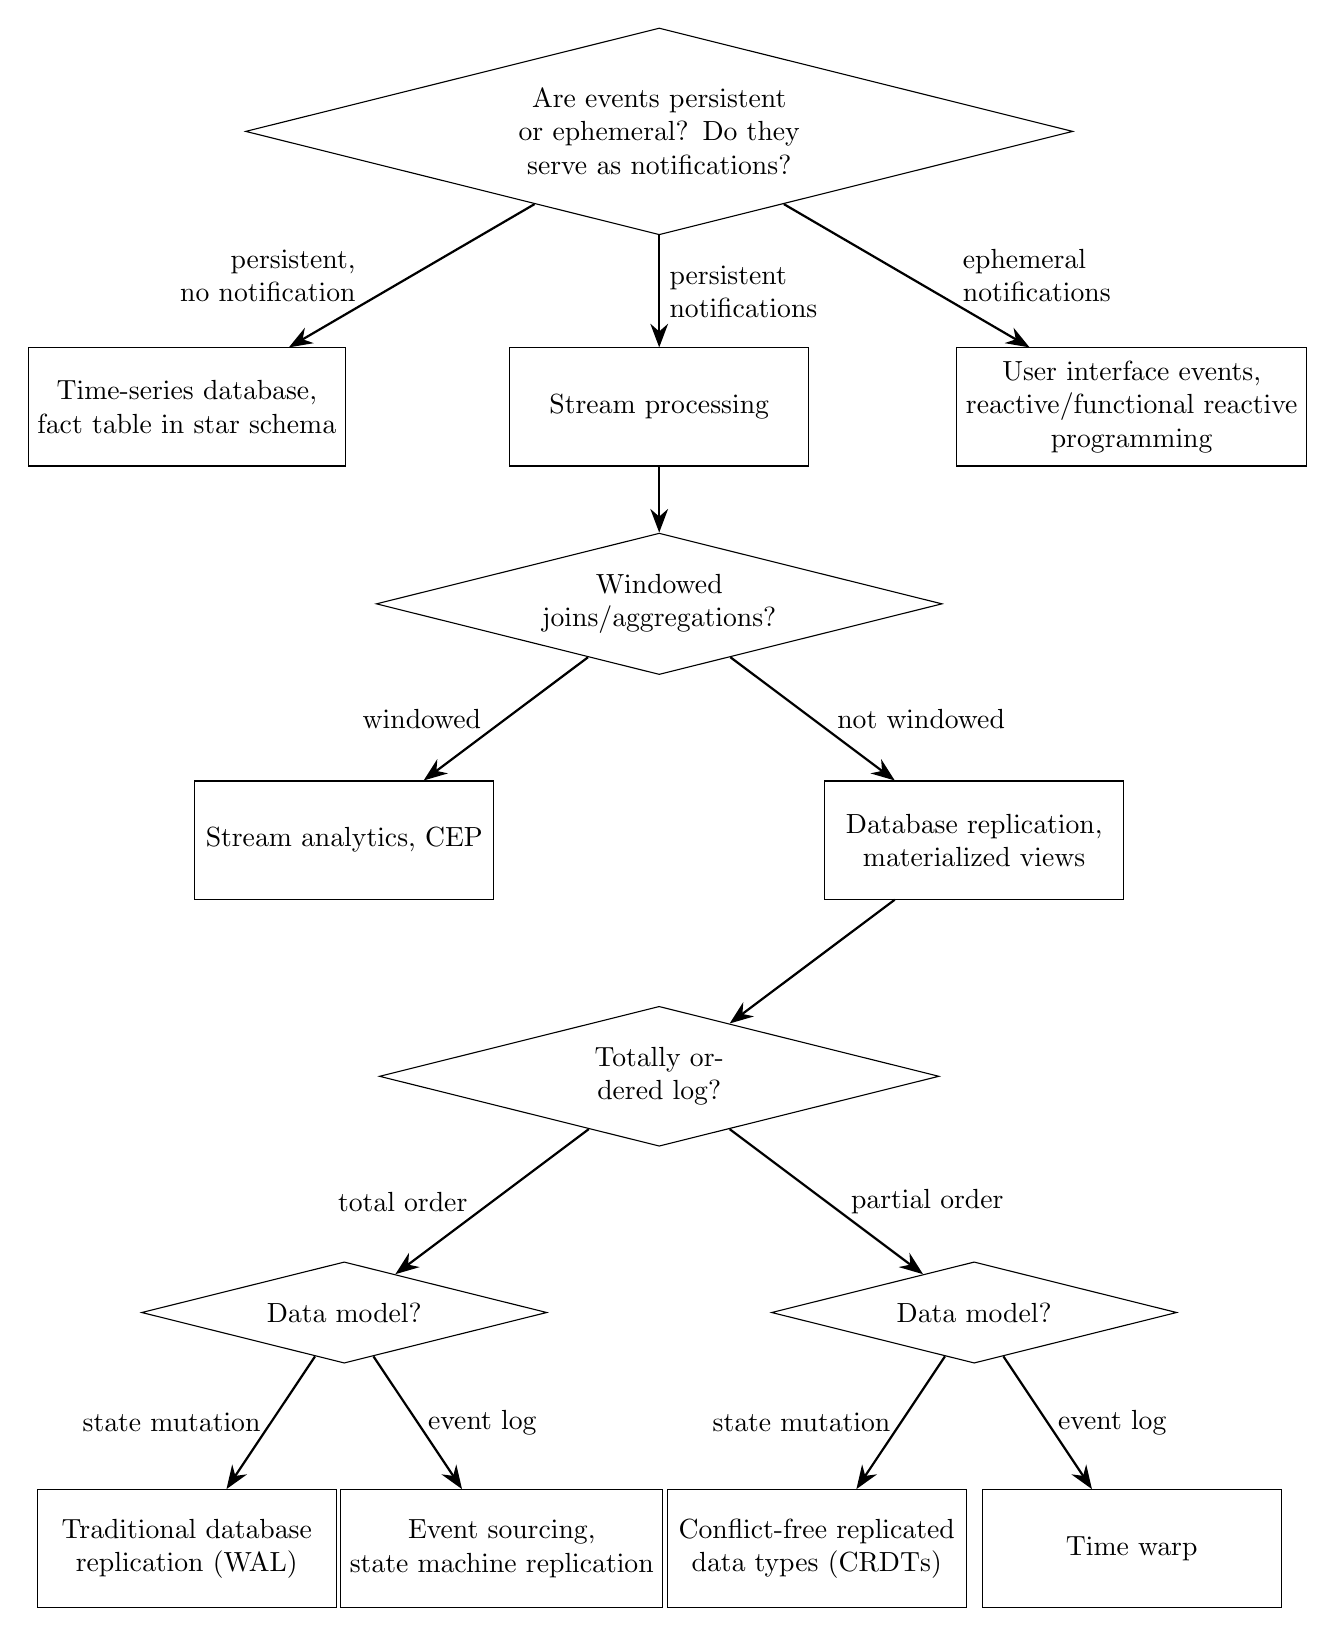
\begin{tikzpicture}
\tikzstyle{question}=[diamond,draw,aspect=4,text width=3cm,align=center]
\tikzstyle{box}=[rectangle,draw,align=center,minimum width=3.8cm,minimum height=1.5cm]
\tikzstyle{arrow}=[{Stealth[length=3mm]}-,thick]
\node [diamond,draw,text width=5cm,align=center,aspect=4] (n1) at (0,0) {Are events persistent or ephemeral? Do they serve as notifications?};
\node (n2) [box] at (-6,-3.5) {Time-series database,\\fact table in star schema} edge [arrow] node [left,align=right,inner xsep=7mm] {persistent,\\no notification} (n1);
\node (n3) [box] at (0,-3.5) {Stream processing} edge [arrow] node [right,align=left] {persistent\\notifications} (n1);
\node (n4) [box] at (6,-3.5) {User interface events,\\reactive/functional reactive\\programming} edge [arrow] node [right,align=left,inner xsep=7mm] {ephemeral\\notifications} (n1);
\node (n5) [question] at (0,-6) {Windowed joins/aggregations?} edge [arrow] (n3);
\node (n6) [box] at (-4,-9) {Stream analytics, CEP} edge [arrow] node [left,inner xsep=3mm] {windowed} (n5);
\node (n7) [box] at (4,-9) {Database replication,\\materialized views} edge [arrow] node [right,inner xsep=3mm] {not windowed} (n5);
\node (n8) [question] at (0,-12) {Totally ordered log?} edge [arrow] (n7);
\node (n9) [question] at (-4,-15) {Data model?} edge [arrow] node [left,inner xsep=3mm] {total order} (n8);
\node (n10) [box] at (-6,-18) {Traditional database\\replication (WAL)} edge [arrow] node [left] {state mutation} (n9);
\node (n11) [box] at (-2,-18) {Event sourcing,\\state machine replication} edge [arrow] node [right] {event log} (n9);
\node (n12) [question] at (4,-15) {Data model?} edge [arrow] node [right,inner xsep=3mm] {partial order} (n8);
\node (n13) [box] at (2,-18) {Conflict-free replicated\\data types (CRDTs)} edge [arrow] node [left] {state mutation} (n12);
\node (n14) [box] at (6,-18) {Time warp} edge [arrow] node [right] {event log} (n12);
\end{tikzpicture}
\centering
\caption{A taxonomy of event-based systems.}
\label{fig:flowchart}
\end{figure*}

\subsection{Notifications and persistence}

At a high level, an event can be:
\begin{itemize}
\item a notification about the fact that something happened;
\item a persistent record of the fact that something happened; or
\item both.
\end{itemize}

Examples of notification events occur in many applications.
JavaScript code running in a web browser can register functions to be called when the user does something, such as clicking or typing a key on the keyboard: here the click or the key-press is the event.
Most other user interface frameworks have a similar system of dispatching user input events to callback functions or \emph{event handlers}.
Many operating systems offer asynchronous (non-blocking) I/O functionality, in which case a thread runs an \emph{event loop} that processes notifications from the OS when requested I/O operations complete.
Reactive and functional reactive programming (FRP) offer higher-level APIs, such as a dataflow programming model, for working with \emph{streams of events}.
In all of these examples, an event is something that exists only in-memory in a single process; it is ephemeral, not persistent, in the sense that it is not normally written to disk.
Ephemeral events exist only for the lifetime of a process and are not preserved across restarts.

In contrast, persistent events do not necessarily have a notification element.
For example, time-series databases are often used to record events that occurred over time, such as periodic readings from a sensor, price updates of a financial asset, and tracking the activity of a person or machine.
Another example is the fact table that appears in the star or snowflake schema of data warehouses and business analytics systems: every row in the fact table is typically a timestamped record of an event that happened, such as the purchase of a particular product by a particular customer.
In such systems, an event is a value that is recorded in a database for future analysis, but the receipt of the event does not necessarily trigger the immediate execution of any application code.
The primary purpose of the events from the user's point of view is to allow the retroactive querying and analysis of the event history, such as examining trends and generating reports showing the change of some metric over time.

Some systems combine these characteristics such that an event is both a persistent record of the fact that something happened, and also a notification (i.e.\ application code is called to handle the occurrence of an event).
I will broadly group such systems under the term \emph{stream processing}, and break them down into subcategories later.
Some databases provide facilities such as \emph{materialized view maintenance} and \emph{continuous queries} (queries whose results are automatically updated as the underlying data changes), which can also be regarded as a form of notification.

Many programming models for distributed systems are based on sending and receiving messages, and the receipt of a message can also be seen as a notification event that triggers the execution of application code.
For example, the \emph{actor model} is a widely-used approach in which multiple actors or lightweight threads, potentially located on different machines, communicate by sending each other messages.
In many distributed systems these messages are ephemeral (they might be lost if a part of the system crashes or if the network is unreliable), but some actor frameworks and messaging middleware systems also include persistence mechanisms for actor state and/or messages.
For the purposes of this taxonomy I will reserve the term ``persistent'' for those systems in which message delivery is reliable, data is durable, and all state in the system is preserved in case of a crash or network fault; any systems with best-effort message delivery fall into the ``ephemeral notifications'' category.

\subsection{Windowing in stream processing}\label{sec:windowing}

Zooming in on the systems that provide both persistence and notifications, we can further differentiate them by examining the kind of logic that can be performed in response to an event.
The very simplest stream processors use stateless operators, in which every event can be processed independently of any other event, based only on the information in that event (for example, selecting events where a certain property of the event falls within some set of values).
However, stateless processing is rarely sufficient, and most interesting applications also require event processing logic that combines information from several events: in database parlance, a \emph{join} or \emph{grouping} of events.
Events may be combined by aggregation (e.g.\ computing the count, sum, or average of some property of a set of events), by emitting compound events that include properties from several input events, or by more complex state machines that we discuss in \autoref{sec:smr}.

Some stream processing systems are designed primarily for applications in which the events that need to be combined occur fairly close together in time.
For example, a stock trading system may need to compute the minimum and maximum prices of an asset per hour or per day, or a fraud detection system may need to detect unusual patterns of recent activity on a customer's credit card.
Such operations are known as \emph{windowed} joins or aggregations.
Several types of window are in use (such as tumbling or sliding windows), but they all have in common that they place a bound on the maximum time interval between any two events that may be combined; any events that are further apart in time than this bound are treated as unrelated.
Windowed processing often occurs when performing business analytics on streams, or in \emph{complex event processing} (CEP).

On the other hand, some applications need to combine events that may lie arbitrarily far apart in time, and thus windowing is not applicable.
For example, imagine a Twitter-like social network in which users may post messages and update their profile photo.
Posting a message is one type of event, and updating the photo is another type of event.
Now say that for display purposes we want to attach the sender's most recent profile photo to every message-posting event.
It may well be that the user last updated their profile photo years ago, and thus, finding the current photo requires going back arbitrarily far in the stream of profile photo update events.

In a SQL database, this join between messages and profile photos might be expressed as follows:

\begin{minted}{sql}
SELECT messages.*, profiles.photo_url
FROM messages
JOIN profiles ON messages.sender_id = profiles.user_id
\end{minted}

The message-posting event in an event-based system corresponds to inserting a row into this \texttt{messages} table, and the photo-updating event corresponds to updating the user's entry in the \texttt{profiles} table.
A stream processor that combines these events is effectively acting as a continuous query execution engine that maintains the output of the query above, i.e.\ maintaining a materialised view of the query.
It may perform the join using a database that contains the most recent profile photo per user, updating that database on every photo-updating event, and querying that database on every message-posting event.

One detail that such a system needs to decide is: when a user updates their profile photo, do we go back and retroactively attach the most recent photo to all of the user's past messages, or do we attach the new profile photo only to messages posted after the photo change?
The query above seems to suggest the former, and this is also what Twitter does in practice, but this means that the stream processor needs to be able to scan over the entire history of past message-posting events when a photo-updating event is received.
The latter policy might also be reasonable: it would be easier to implement in imperative code, but more complicated to express in SQL.

\subsection{Database replication and events}\label{sec:replication}

If we focus our attention on systems where the events are persistent notifications without windowing, we may notice a strong similarity to replication in database systems.
The goal of replication is to have a copy of the same data on several different machines: that is, any two replicas converge to the same state, and all committed transactions are reflected in that state.
Viewed through the lens of event-based systems, we can treat every transaction that modifies the database as an update event, the execution of an update (i.e.\ reflecting the update in the database state) as the processing of that event, and the replication of data from one machine to another as the propagation of that event through the distributed system.
Read-only transactions may or may not correspond to events, depending on the system.

In such a database system, the replication infrastructure ensures that every event corresponding to a committed transaction is eventually processed by every non-faulty replica.
We can classify such replication systems into two broad categories: those that arrange the replication events into a log, and those that use some other replication mechanism (such as gossip protocols, anti-entropy, or clients independently updating several replicas).
The key properties of a log are that the events in it are totally ordered (i.e.\ all replicas observe the log entries in the same order), and it is append-only (i.e.\ if a replica observes log entry $A$ immediately followed by log entry $B$, then there will never be a log entry $C$ that appears between $A$ and $B$ in the total order).

This append-only log is constructed either using a consensus protocol such as Raft or Multi-Paxos, or by designating one replica as the \emph{leader} (also known as master or primary) and all other replicas as followers (aka slaves or secondary replicas).
In fact, most consensus protocols are essentially leader-based replication combined with an automatic mechanism for electing a new leader if the current leader fails.
The leader decides on the order in which events should be appended to the log, and all other replicas process the events in the order decided by the leader.

In many databases, the exact structure and content of the events in the log has traditionally been an implementation detail of the database system that is not exposed to applications.
For example, several database systems use the \emph{write-ahead log} (WAL) for replication, which consists of records indicating how the database's on-disk data structures are changing; others use a separate replication log.
More recently, \emph{change data capture} techniques have been developed to extract the data change events (rows inserted, updated, or deleted) from this log and make them available to applications via stream processing systems.

\subsection{State machine replication (SMR)}\label{sec:smr}

In WAL-based replication and change data capture, the primary data model used by the application is the database state that can be mutated by the application (e.g.\ by inserting, updating, or deleting rows in tables), and the data change events are generated automatically as a side-effect of these mutations.
It is also possible to swap these roles, making the data change events the primary data model of the application, so that any state changes become a side-effect of processing those events.
This is the idea behind \emph{state machine replication}~\cite{Schneider:1990}, and the closely related concept of \emph{event sourcing}~\cite{Fowler:2005}.

In state machine replication (SMR) and event sourcing, the application does not directly mutate the state of a database.
Instead, the application defines a set of event types that may occur, and whenever something happens, an event of the appropriate type is appended to an event log.
All replicas subscribe to this event log, and each replica processes events in the order in which they appear in the log.
The event processing function can use arbitrary logic to update the database state, as long as it is deterministic and it depends only on the current database state and the content of the event.
Provided that each replica processes the same sequence of events in the same order, and each replica starts in the same initial state (e.g.\ an empty database), the deterministic event processing logic ensures that all replicas move through the same sequence of states and end up in the same final state.
We can think of each replica as a state machine whose state is its copy of the database, and whose state transition function is the event processing function.
Put another way, the database state is a materialised view onto the underlying event log.

An advantage of this approach is that well-designed events often capture the intent and meaning of operations better than events that are a mere side-effect of a state mutation.
For example, ``student $x$ cancelled their enrollment in course $y$ for reason $z$'' is a clear descriptive event, whereas ``one row was deleted from the \verb+enrollments+ table, one row was added to the \verb+cancellation_reasons+ table, and the \verb+available_places+ field of a course was incremented'' is a much less clear description that embeds a lot of irrelevant detail about the current database schema.
An event log thus makes it easier for the people who work with a system to understand how it got into a particular state, which can help with audit and debugging.

Another advantage of an event log is that it can be replayed in order to rebuild the resulting database state.
If the application developers wish to change the logic for processing an event, for example to change the resulting database schema or to fix a bug, they can set up a new replica, replay the existing event log using the new processing function, switch clients to reading from the new replica instead of the old one, and then decommission the old replica.
This sort of retroactive change in business logic is not usually possible in state-mutation databases.
It is easy to maintain several different views onto the same underlying event log if needed.
As long as the rate of updates is not too high, it is often feasible to retain the event log indefinitely and replay it occasionally as needed.

Blockchains and distributed ledgers also use SMR, in which case the chain of blocks (and the transactions therein) constitutes the event log, the ledger (e.g.\ the balance of every account) is the resulting state, and smart contracts or built-in transaction processing logic are the state transition function.

The downside of the event sourcing/SMR approach is that it is less familiar to most application developers than mutable-state databases, and the level of indirection between the event log and the resulting database state adds complexity in some types of applications that are more easily expressed in terms of state mutations.

\subsection{Partially ordered events}\label{sec:partial-order}

Both WAL-based replication and SMR depend crucially on the assumptions that all replicas process events in exactly the same order.
Within a single datacenter, this is a reasonable assumption, since leader-based replication and consensus protocols work well in this setting.
However, if replicas are distributed across multiple geographic locations, or if the network between replicas is unreliable, constructing a log becomes expensive, since appending an event to the log requires at waiting least one network round-trip to the leader and/or a quorum of replicas.
In the extreme case, if we want a replica to be able to generate and process events even while it is completely disconnected from all other replicas (a system that is ``available'' and ``partition-tolerant'' in the sense of the CAP theorem~\cite{Gilbert:2002}), the assumption of a totally ordered log becomes impossible to satisfy.

In a system that allows disconnected operation, the strongest order we can guarantee is causal order~\cite{Attiya:2015}.
This is a \emph{partial} order, in contrast to the total order of a log.
In a causally ordered system, some events \emph{happened before} other events~\cite{Lamport:1978}, and those events are processed in the same order by all relicas.
However, other events may be \emph{concurrent}, which means that neither happened before the other; in this case, different replicas may process those events in a different order.

\begin{figure*}
  \centering\vspace{2em}
  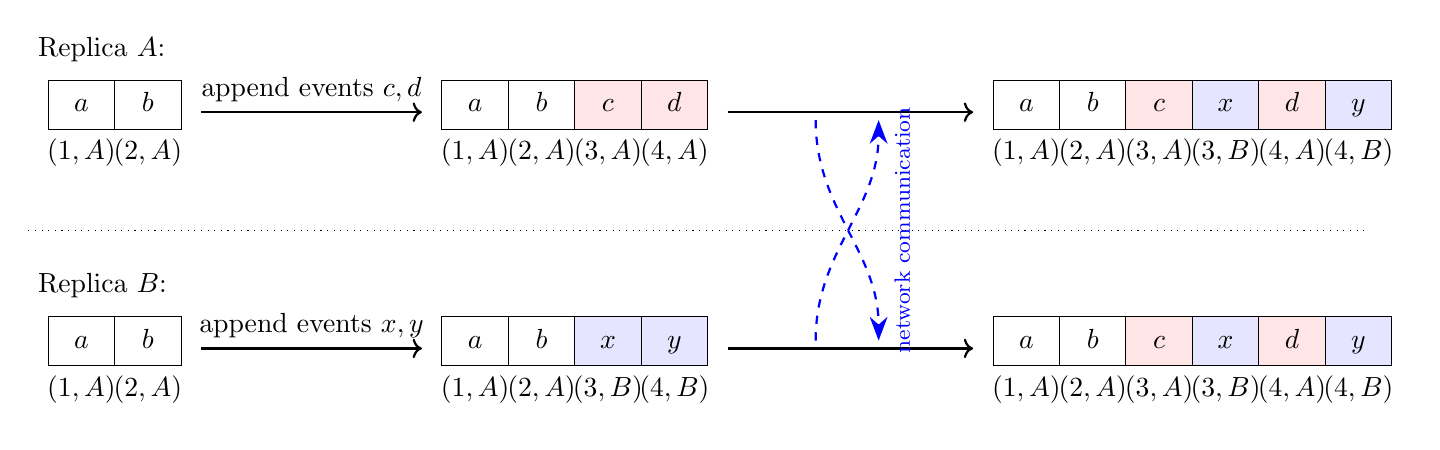
\begin{tikzpicture}[auto,scale=1.0]
	\tikzstyle{state}=[matrix,column sep={24pt,between origins},anchor=west]
	\tikzstyle{val}=[draw,anchor=base,minimum width=24pt,text height=8pt,text depth=3pt]
	\tikzstyle{oid}=[anchor=base]
	\tikzstyle{ins1}=[fill=red!10]
	\tikzstyle{ins2}=[fill=blue!10]
	\tikzstyle{time}=[thick,->]
	\tikzstyle{network}=[thick,dashed,blue,-{Stealth[length=3mm]}]
	\node at (0,4) [anchor=west] {Replica $A$:};
	\node at (0,1) [anchor=west] {Replica $B$:};
	\node (a1) at (0,3) [state] {
		\node [val] {$a$}; &
		\node [val] {$b$}; \\
		\node [oid] {$(1,A)$}; &
		\node [oid] {$(2,A)$}; \\
	};
	\node (b1) at (0,0) [state] {
		\node [val] {$a$}; &
		\node [val] {$b$}; \\
		\node [oid] {$(1,A)$}; &
		\node [oid] {$(2,A)$}; \\
	};
	\node (a2) at (5,3) [state] {
		\node [val] {$a$}; &
		\node [val] {$b$}; &
		\node [val,ins1] {$c$}; &
		\node [val,ins1] {$d$}; \\
		\node [oid] {$(1,A)$}; &
		\node [oid] {$(2,A)$}; &
		\node [oid] {$(3,A)$}; &
		\node [oid] {$(4,A)$}; \\
	};
	\node (b2) at (5,0) [state] {
		\node [val] {$a$}; &
		\node [val] {$b$}; &
		\node [val,ins2] {$x$}; &
		\node [val,ins2] {$y$}; \\
		\node [oid] {$(1,A)$}; &
		\node [oid] {$(2,A)$}; &
		\node [oid] {$(3,B)$}; &
		\node [oid] {$(4,B)$}; \\
	};
	\node (a3) at (12,3) [state] {
		\node [val] {$a$}; &
		\node [val] {$b$}; &
		\node [val,ins1] {$c$}; &
		\node [val,ins2] {$x$}; &
		\node [val,ins1] {$d$}; &
		\node [val,ins2] {$y$}; \\
		\node [oid] {$(1,A)$}; &
		\node [oid] {$(2,A)$}; &
		\node [oid] {$(3,A)$}; &
		\node [oid] {$(3,B)$}; &
		\node [oid] {$(4,A)$}; &
		\node [oid] {$(4,B)$}; \\
	};
	\node (b3) at (12,0) [state] {
		\node [val] {$a$}; &
		\node [val] {$b$}; &
		\node [val,ins1] {$c$}; &
		\node [val,ins2] {$x$}; &
		\node [val,ins1] {$d$}; &
		\node [val,ins2] {$y$}; \\
		\node [oid] {$(1,A)$}; &
		\node [oid] {$(2,A)$}; &
		\node [oid] {$(3,A)$}; &
		\node [oid] {$(3,B)$}; &
		\node [oid] {$(4,A)$}; &
		\node [oid] {$(4,B)$}; \\
	};
	\draw [time] ([yshift=2mm]a1.east) -- node [above] {append events $c,d$} ([yshift=2mm]a2.west);
	\draw [time] ([yshift=2mm]a2.east) -- ([yshift=2mm]a3.west);
	\draw [time] ([yshift=2mm]b1.east) -- node [above] {append events $x,y$} ([yshift=2mm]b2.west);
	\draw [time] ([yshift=2mm]b2.east) -- ([yshift=2mm]b3.west);
    \draw [network] (10,3.1) to [out=270,in=90] (10.8,0.3);
    \draw [network] (10,0.3) to [out=90,in=270] (10.8,3.1);
	\node [blue,rotate=90,font=\footnotesize] at (11.1,1.7) {network communication};
	\path [draw,dotted] (0,1.7) -- (17,1.7);
  \end{tikzpicture}
  \caption{Obtaining a total order on events using Lamport timestamps, which are $(\mathit{counter}, \mathit{replicaID})$ pairs. Two events with the same $\mathit{counter}$ are ordered by $\mathit{replicaID}$; here we assume that $A<B$.}
  \label{fig:timestamp-order}
\end{figure*}

In a partially ordered system it is still possible to enforce a total order on events after the fact, as illustrated in \autoref{fig:timestamp-order}.
We do this by attaching a logical timestamp to each event; Lamport timestamps~\cite{Lamport:1978} are a common choice.
These timestamps consist of a counter, which is incremented for every event, together with the globally unique ID of the replica that generated the event.
In \autoref{fig:timestamp-order}, two replicas initially have the same two events $a$ and $b$ with timestamps $(1,A)$ and $(2,B)$ respectively.
During a period when the two replicas are disconnected from each other, replica $A$ generates two events $c$ and $d$ with timestamps $(3,A)$ and $(4,A)$ respectively, while concurrently replica $B$ generates events $x$ and $y$ with timestamps $(3,B)$ and $(4,B)$.
After connectivity is restored, the replicas learn about each others' events, and merge them into a total order.
This order is defined by first sorting events by the counter portion of their timestamps, and then breaking ties by sorting by replica ID (here we assume $A<B$).

Timestamp ordering produces a totally ordered sequence of events, but it is not a log, because new events are not always appended to the end.
In \autoref{fig:timestamp-order}, when replica $B$ receives event $c$ from $A$, it must insert $c$ ahead of its existing events $x$ and $y$ in its event sequence.
Similarly, replica $A$ must insert $x$ between its existing events $c$ and $d$.
In SMR, the total order of events is fixed as soon as an event is processed, but with timestamp ordering, the order may need to be revised as more events are received from other replicas.

It is possible to use timestamp-ordered events in an SMR-like approach: that is, to use a deterministic function to apply events one by one to the current replica state.
Assuming every replica eventually receives every event, all replicas will eventually have the same timestamp-ordered sequence of events, and thus all replicas will go through the same sequence of states and end up in the same state.
However, when a replica processes events out of timestamp order (inserting an event somewhere in the middle of the timestamp-ordered sequence), it must be able to roll back the replica state to the time corresponding to the insertion position, apply the new event, and then replay the events whose timestamps are greater than that of the new event.
This approach is known as \emph{time warp}~\cite{Jefferson:1985}.

The cost of this rollback-and-replay process depends on the degree to which events are received out-of-order.
If the replicas receive most events in ascending timestamp order, and they only occasionally need to reorder the most recent couple of events, the cost can be modest~\cite{Kuhn:2021}.
On the other hand, if replicas might generate large numbers of events while disconnected from each other, the cost of merging $n$ events into a linear sequence may become as great as $O(n^2)$.

Moreover, if processing an event may have external side-effects besides updating a replica state~-- for example, if it may trigger an email to be sent~-- then the time warp approach requires some way of undoing or compensating for those side-effects in the case where the processing of an event is affected by a late-arriving event with an earlier timestamp.
It is not possible to un-send an email once it has been sent, but it is possible to send a follow-up email with a correction in this case.
If the possibility of such corrections is unacceptable, partially ordered events cannot be used, and SMR must be used instead.

\subsection{Conflict-free Replicated Data Types (CRDTs)}\label{sec:crdts}

In the time warp approach, like in SMR/event sourcing, the events are the primary data model for the application, and the replica state is derived from the events.
Similarly to \autoref{sec:smr}, we can also choose to swap these roles, so that the mutable replica state is the application's primary data model, and the events are generated automatically as a side-effect of mutating this state.
If we take the mutable-state approach in the context of a partially ordered system, we obtain a technique called \emph{Conflict-free Replicated Data Types} or CRDTs~\cite{Shapiro:2011}.

CRDTs have been defined for a number of common abstract data types: sets, maps, lists, trees, graphs, and so on.
Applications may mutate these structures through the operations provided by the data type's interface: for example, a set or a list can be mutated by inserting or deleting elements; a map can be mutated by assigning a value to a key or by deleting a key-value pair.
These mutations can take place even while a replica is disconnected from the rest of the system.

In operation-based CRDTs, the CRDT algorithm tracks any mutations to a data object and generates events (usually called ``operations'') describing the changes.
These events are partially ordered; causal ordering, like in \autoref{sec:partial-order}, is a common choice.
When a replica receives an event generated by another replica, it invokes the CRDT algorithm to update its state.
This algorithm is carefully designed such that applying concurrent events is commutative: that is, the final state is the same, regardless of the order in which a replica applies a set of concurrent events.

Many CRDT algorithms have behaviour that can equivalently be expressed in the time warp model~\cite{Kleppmann:2018}.
However, CRDTs have the advantage that they usually do not require the rollback-and-replay process of time warp, so they can offer higher performance~\cite{dePorre:2019}.
A disadvantage of CRDTs is that they support only the predefined operations offered by the data type's interface: for example, while list CRDTs allow elements to be inserted or deleted, most do not have good support for reordering list items~\cite{Kleppmann:2020}.
In contrast, the time warp model allows any deterministic, pure function to be used for processing events, making it more flexible.

\begin{figure*}
\centering
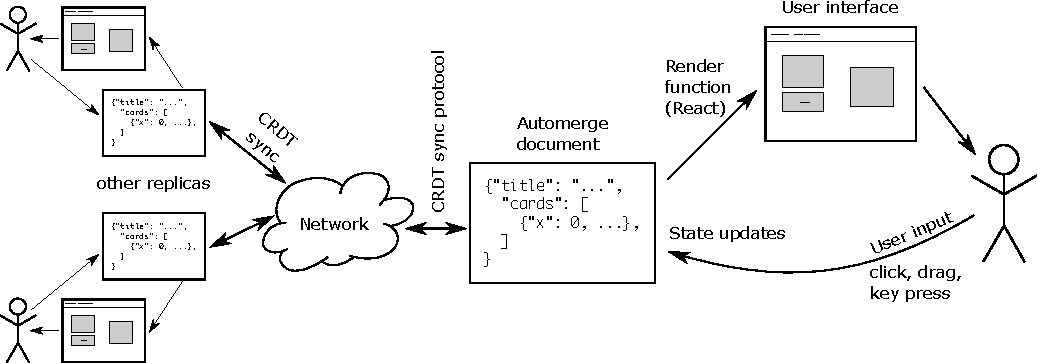
\includegraphics{document-frp.pdf}
\caption{A functional reactive programming model for local user input and collaboration with remote users. Figure from \cite{vanHardenberg:2020}.}
\label{fig:pushpin}
\end{figure*}

\section{Practical Examples}

I will close with a personal perspective by briefly discussing practical applications of the models from \autoref{sec:taxonomy}.
I draw examples from two areas I have directly worked on: stream processing with Apache Kafka and related tools, and collaboration software that allows several people to work together on a shared document.

\subsection{The Kafka Ecosystem}

TODO

\subsection{Local-first Collaboration Software}

Over the past several years, my collaborators and I have been working on new foundations for collaboration software, that is, applications that allow several users to collaboratively modify a shared file.
The file could be a text document, a drawing, a spreadsheet, a to-do list, or many other types of data.
Software that runs on mobile devices needs to work offline: for example, you should be able to add an item to your to-do list even if your phone currently has no cellular data coverage.
It is therefore clear that this type of application operates in the partially ordered, non-windowed, persistent part of the taxonomy.

More specifically, we are designing this software according to the \emph{local-first} approach~\cite{Kleppmann:2019}, in which every end-user device from which a user accesses their data is treated as a full-fledged replica using its local on-device storage.
When a user modifies their data, they immediately update the replica on their local device, even if it is offline, and any updates are synced to the replicas on other users' devices the next time a network connection is available.

We use CRDTs to implement this approach, and thus the events describing data updates are generated by the CRDT algorithm as a side-effect of a mutation of a replica's state.
This model is a good fit for collaboration software because the user input takes the form of state mutations: for example, in a text document, a user needs to be able to insert or delete characters anywhere in the document.
Moreover, what the user wants to see on screen is usually the current state of the document, not a log of all of the change events (although visualised change history is a useful feature too).
To this end we have developed a CRDT library called Automerge,\footnote{\url{https://github.com/automerge/automerge}} which provides a JSON data model.

CRDT-generated events also serve as notification that a document has changed, which enables real-time collaboration among several users editing the same document.
We handle such events using a \emph{functional reactive programming} model illustrated in \autoref{fig:pushpin}.
The current state of the user's application is represented as an Automerge CRDT data structure.
A rendering function takes this data structure and translates it into the corresponding user interface elements that should be displayed on screen~\cite{vanHardenberg:2020}.
In web applications, Facebook's React\footnote{\url{https://reactjs.org/}} is a popular library for performing this kind of rendering.

The rendered user interface has attached event handlers that are called when the user interacts with the respective user interface elements (these events are ephemeral).
When such an event handler is called, it does not update the user interface directly, but rather it mutates the Automerge state to reflect the user input, and then the rendering function is called again to update the user interface.
This functional reactive programming model makes the software easy to reason about, because data flows only one way: the user interface state is always derived from the Automerge state, not the other way around.

When a user thus mutates the Automerge state, the CRDT generates a change event, persists it locally, and uses a messaging middleware or sync protocol to send it to all other devices that have a replica of that document.
When a replica receives such an event from a remote user, it uses the CRDT logic to update the local Automerge state, and then calls the rendering function in exactly the same way as it does for a change made by the local user.
Using the same code paths and data flows for real-time collaboration as for local user input significantly simplifies the programming model.

This approach is discussed in more detail in our prior paper on PushPin~\cite{vanHardenberg:2020}, one of our local-first software prototypes.

\section{Conclusions}

TODO

\bibliographystyle{ACM-Reference-Format}
\bibliography{references}{}

\end{document}
